\subsection{Experimental estimation of damping}
\label{se:experimental_estimation}

The ordinary differential equations for roll motion in equation \ref{eq:roll_decay_equation_cubic}, \ref{eq:roll_decay_equation_himeno_quadratic} and
\ref{eq:roll_decay_equation_himeno_linear} are solved numerically using Explicit Runge-Kutta method of order 5(4). Figure \ref{fig:analytical} shows a comparison for the linear model between this kind of numerical solution and the exact analytical solution \cite{henry_peter_piehl_ship_nodate}. It seems that the numerical solution agrees well with the analytical. 

\begin{figure}[h]
    \centering
    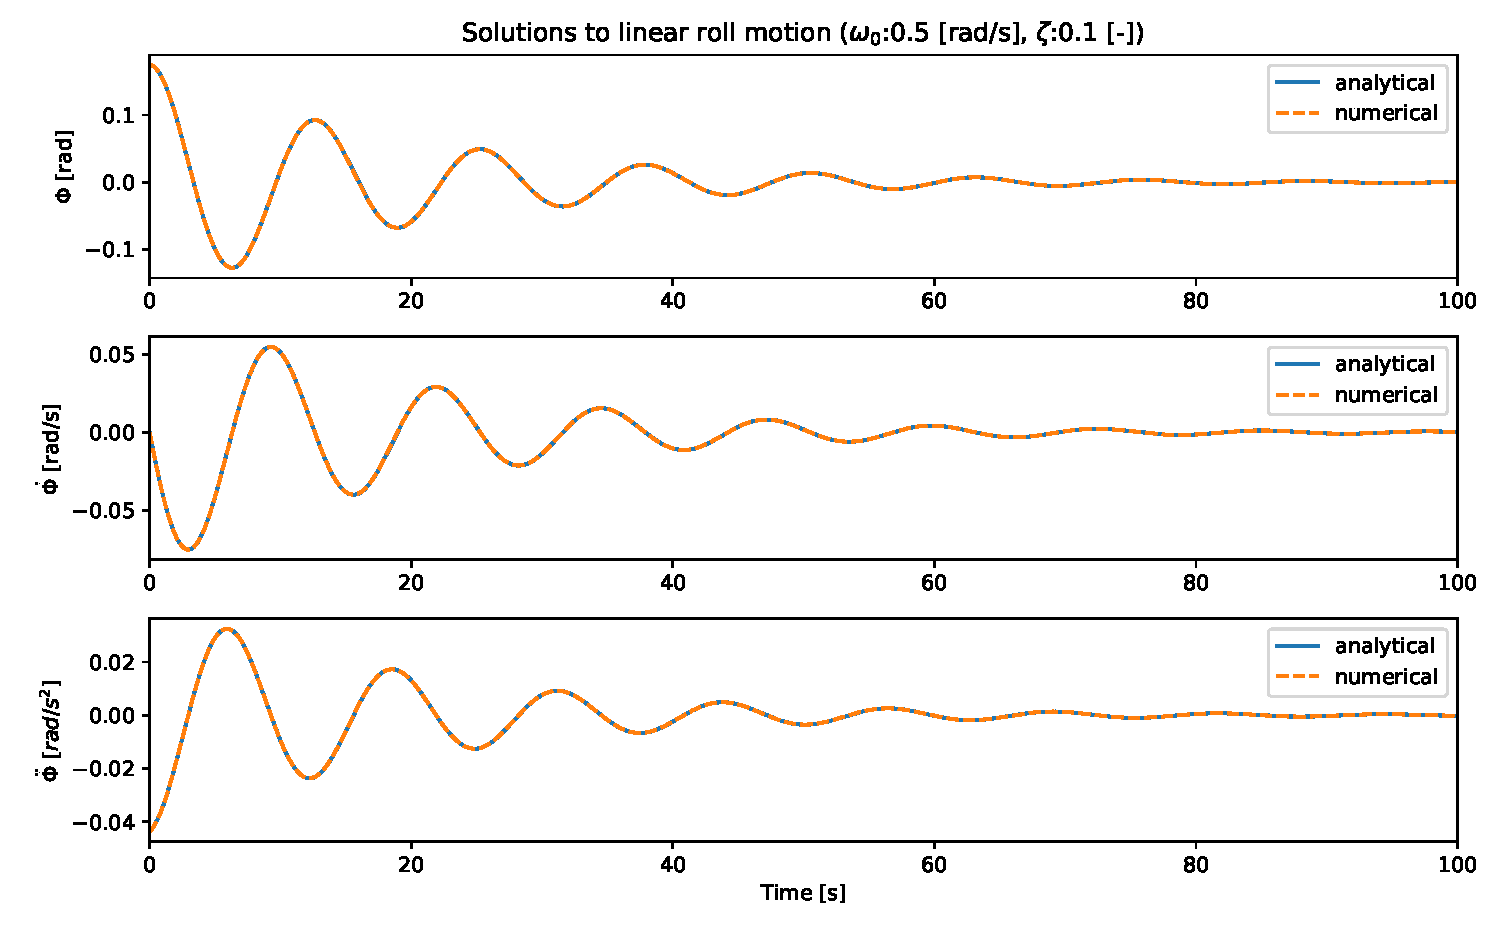
\includegraphics[width=\columnwidth]{figures/analytical.pdf}
    \caption{Analytical and numerical solution to the linear model}
    \label{fig:analytical}
\end{figure}


\subsection{Parameter Identification Technique}
\label{se:PIT}
In order to extract roll damping parameters from the roll decay tests, parameters in the cubic, quadratic or linear roll decay models should be identified. The roll angle is measured during the roll decay tests. The system identification is defined as finding the parameters that produce a simulated roll signal that best fits the roll decay test measurement. The goodness of the fit is described using the coefficient of determination:
\begin{equation} \label{eq:R2}
R^2=1-\frac{SS_{res}}{SS_{tot}}
\end{equation}
Where $SS_{res}$ is sum of squares of residuals and $SS_{tot}$ is total sum of squares. Two different solution approaches have been investigated for the system identification: a "Derivation approach" and an "Integration approach". 

In the "Derivation approach" the first and second roll time derivatives are calculated numerically so that the parameters in the models are the only unknowns and the optimal parameters that gives the best fit can simply be determined using a least square fit.

In the "Integration approach" the parameters are found by solving a nonlinear least-squares problem using \emph{SciPy} method \emph{least\_squares} \cite{noauthor_scipyoptimizeleast_squares_nodate} and the Trust Region Reflective algorithm with smooth approximation of l1 (absolute value). This approach requires that ordinary differential equation is solved for many "guessed" sets of parameters till the solution converges.

The "Derivation approach" has the advantage of being very much faster than the "Integration approach" but also the disadvantage of needing to calculate the numerical derivatives which for measurement data also requires some low pass filtration. The "Integration approach" may however also have a disadvantage of not converging.

A validation of the developed system identification method has been conducted by checking that known parameters from signals from simulations with the linear, quadratic and cubic models can all be identified. 

Figure \ref{fig:roll_decay_model_compare} shows a comparison between the linear, quadratic and cubic model, where it can be seen that the linear model can not give a perfect representation for the whole range of roll angles.    

\begin{figure}[H]
    \centering
    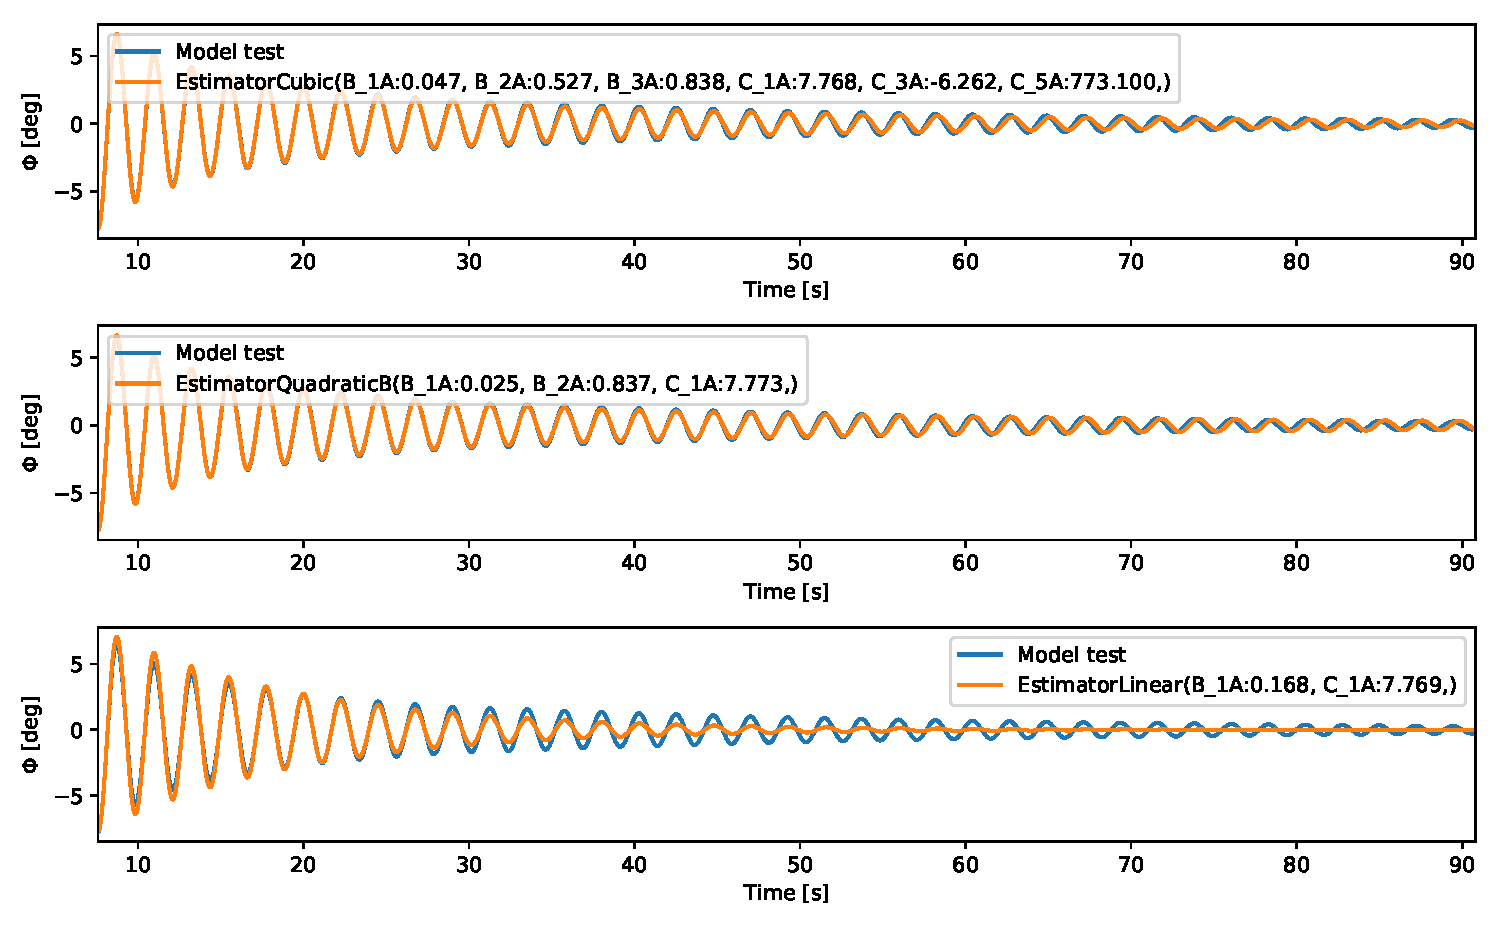
\includegraphics[width=0.9\columnwidth]{figures/roll_decay_model_compare.pdf}
    \caption{Roll decay test comparison of linear, quadratic and cubic model}
    \label{fig:roll_decay_model_compare}
\end{figure}
